\documentclass{article}
\usepackage[utf8]{inputenc}

\title{Homework No.1}
\author{Osamu Katagiri-Tanaka : A01212611}
\date{\today}

\usepackage{enumitem}
\usepackage{geometry}
\geometry{
	paper         = a4paper, % Change to letterpaper for US letter
	inner         = 2.5cm,   % Inner margin
	outer         = 2.5cm,   % Outer margin
	bindingoffset = 0.5cm,   % Binding offset
	top           = 1.5cm,   % Top margin
	bottom        = 1.5cm    % Bottom margin
}
\usepackage{graphicx}
\usepackage[
    style   = ieee,
    backend = biber,
    natbib  = true
]{biblatex}
\addbibresource{references.bib}

\begin{document}

\maketitle

\section*{\emph{What will I achieve?}}
With this homework you will practice the use of the concepts and knowledge acquired throughout the corresponding topics.

\section*{Instructions}

\subsection*{Part A}
\textit{Find five differential equations found in fluid mechanics, heat transfer, mass transfer, bioengineering or reaction engineering. Three of them must be PDE (Partial differential equations), and you must explain each term, the physical meaning of each term, and what they represent.}

\subsubsection*{Bernoulli equation}

\begin{equation}
\frac{P}{\rho} + \frac{v^2}{2} + g z = constant
\end{equation}

\subsubsection*{Conservation of Mass : Continuity Equation}

\begin{equation}
\frac{\partial \rho}{\partial t} + \vec{\nabla} \cdot (\rho \vec{v}) = 0
\end{equation}

The conservation of mass equation
is obtained by replacing $B$ in the Reynolds transport theorem by mass $m$, and $b$ by 1 ($m$ per unit mass = $1$).
\cite{White2011}

\subsubsection*{Conservation of Energy : 1st Law of Thermodynamics}

\begin{equation}
\frac{\partial E}{\partial t} + \vec{\nabla} \cdot (E \vec{v}) = \rho u + \rho \frac{v^2}{2} + g z
\end{equation}

\subsubsection*{Linear Momentum - Cauchy's equation}

\begin{equation}
\frac{\partial}{\partial t} (\rho \vec{v}) + \vec{\nabla} \cdot (\rho \vec{v} \vec{v}) = \rho \vec{g} + \vec{\nabla} \cdot \sigma_{ij}
\end{equation}

\subsubsection*{Linear Momentun : Navier-Stokes Equation}

\begin{equation}
\rho \frac{d \vec{v}}{d t} = - \vec{\nabla} P + \rho \vec{g} + \mu \nabla^2 \vec{v}
\end{equation}









\subsection*{\emph{Part B}}
\textit{Select one problem of any of the fields listed above, and solve it, following the steps given below.}

\begin{enumerate}
\item \textit{Read problem statement, and collect the information that may be needed.}
\end{enumerate}



\begin{enumerate}[resume]
\item \textit{Make a Sketch (Diagram, process flow chart), indicating mass, linear or angular momentum (i.e. forces and torques) and energy interaction, and label each stream and boundaries as well.}
\end{enumerate}



\begin{enumerate}[resume]
\item \textit{List Assumptions and Approximations (sometimes they may be inferred by the sketch, but make them explicit) supported by equations if possible (geometric relationships, or fundamental equations).}
\end{enumerate}



\begin{enumerate}[resume]
\item \textit{Physical Laws (Fundamental Laws) must be written in full form, and terms can be dropped by the right selection of frame of reference, operating conditions, assumptions, simplifications or constraints.}
\end{enumerate}



\begin{enumerate}[resume]
\item \textit{Physical constants should be obtained from a reliable source (knowing this information by heart is always helpful ), geometric relations and formulae must be included as part of your analysis.}
\end{enumerate}



\begin{enumerate}[resume]
\item \textit{Physical transport or thermodynamic properties (Thermodynamic relations) should be evaluated, approximated, calculated or obtained from a reliable source.}
\end{enumerate}



\begin{enumerate}[resume]
\item \textit{Calculations are done including units. Any algebraic manipulation is recommended in few cases, because limits the step 8, but if needed should be done before using numerical values of constants, properties or variables.}
\end{enumerate}



\begin{enumerate}[resume]
\item \textit{Reasoning (Sensitivity analysis, what if), Verification (context), and Discussion should always be part of your answer to any problem, regardless the task requested.}
\end{enumerate}



\printbibliography[title={References}]
\end{document}

%\begin{figure}[h!]
%\centering
%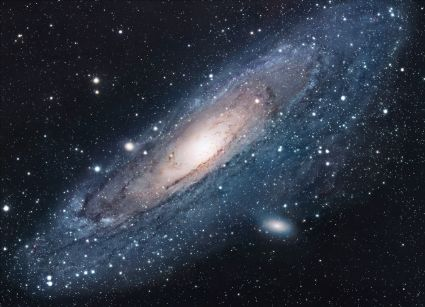
\includegraphics[scale=1.7]{universe}
%\caption{The Universe}
%\label{fig:universe}
%\end{figure}